\documentclass[dvisvgm]{article}
\usepackage{pgfplots}
\usepackage{tikz}
\pgfplotsset{compat=1.16}
\newenvironment{svggroup}[3]{\special{dvisvgm:raw <g data-owns-id="#1" aria-label="#2" data-owns="#3">}}{\special{dvisvgm:raw </g>}}

\usetikzlibrary {arrows.meta,trees}

\begin{document}
\thispagestyle{empty}
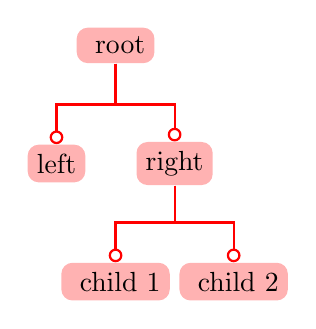
\begin{tikzpicture}[edge from parent fork down,sibling distance=15mm,level distance=15mm,every node/.style={fill=red!30,rounded corners},edge from parent/.style={red,-{Circle[open]},thick,draw}]

\begin{svggroup}{graph}{A rooted graph with two children and 4 descendants}{root}
\node{\begin{svggroup}{root}{root with two children}{left right} root\end{svggroup}}
  child{node{\begin{svggroup}{left}{left node, leaf}{}left\end{svggroup}}}
  child{node{\begin{svggroup}{right}{right node, two children}{child1 child2}right\end{svggroup}}
    child{node{\begin{svggroup}{child1}{child 1, leaf}{} child 1\end{svggroup}}}
    child{node{\begin{svggroup}{child2}{child 2, leaf}{} child 2\end{svggroup}}}
    };
    \end{svggroup}
\end{tikzpicture}

\end{document}
